
\subsection{Feature selection}

Machine learning methods have a difficulty in dealing with the large number of input features and, therefore, pre-processing of the data is essential to use these methods effectively. Feature selection is an important technique which has become indispensable in the machine learning process. It consists in   the process of detecting relevant features and removing irrelevant, redundant, or noisy data. This technique greatly speeds up machine learning algorithms, also improving predictive accuracy and comprehensibility.

There are three feature selection approaches: filters, wrappers and embedded methods. The filter approach incorporates an independent measure for evaluating features subsets without involving a learning algorithm. This method can, however, miss features that are not useful alone but can be very useful in combination with others. On the other hand, the wrapper approach uses a learning algorithm for subset evaluation. This method thus selects an optimal subset that is best suited to the learning algorithm having, therefore, a better performance when compared to the filter approach in most cases. Embedded methods have been recently proposed and try to combine the advantages of both previous methods. In this method, the learning algorithm takes advantage of its own variable selection process and performs feature selection and classification simultaneously \citep{kumar2014feature}. A graphical representation of filter, wrapper and embedded approaches is shown in \autoref{feature_selection}.


\begin{figure}[!htb]
	\centering
	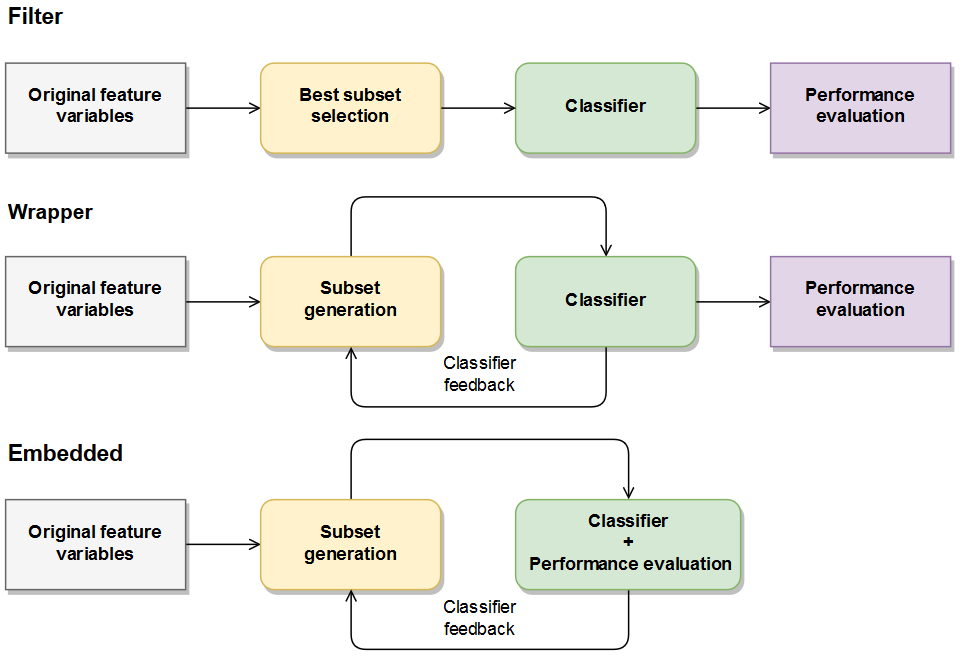
\includegraphics[width=0.85\linewidth]{Imagens/feature_Selection}
	\caption{Workflow of Filter, Wrapper and Embedded approaches in feature selection.}
	\label{feature_selection}
\end{figure}

Filter approaches are based on statistical tests (e.g. chi-squared test) measuring some intrinsic properties of the dataset (or features), including information gain, variance threshold and the correlation coefficient. The latter method was used for instance in the predictive biomarker discovery in biological samples \citep{grissa2016feature}.

Wrapper methods include \gls{rfe}, \gls{sfs} algorithms and \gls{ga}. The \gls{rfe} method uses all initial features to fit the model, ranking all features according to their contribution. In each subset, most relevant variables are retained and the model is refitted. This process continues until the subset with best performance is obtained. While the \gls{rfe} method uses the feature weight coefficients or feature importance, the \gls{sfs} method removes (or adds) features based on a user-defined classifier/regression performance metric, until a feature subset of the desired size k is reached. 

\gls{ga}s are metaheuristic optimization algorithms that use an initial population of candidate solutions (individuals), which is then evolved toward better solutions. This is done by an iterative process, where in each iteration (generation) the fitness (i.e. value of the objective function) of every individual in the population is evaluated. The fittest individuals are stochastically selected from the current population and recombined to form a new generation. The algorithm terminates when either a maximum number of generations has been produced, or a satisfactory fitness level has been reached for the population. This method was used for instance in bacteria discrimination using \gls{ftir} spectroscopy \citep{preisner2007fourier}.

Embedded methods use for instance decision trees and the \gls{lasso} regression algorithm for generalized linear models. \gls{lasso} penalizes the absolute size of the regression coefficients (i.e. forces their sum to be less than a fixed value), which forces certain coefficients to be set to zero. It is a convenient method for automatic feature selection when dealing with highly correlated predictors. This method has been applied for instance in the diagnosis of insulin resistance \citep{milburn2013application}.




